\chapter{Motivation After the Exit}

This source interview from School of Hard Knocks, curated by LazyingArt LLC through Video2Book, gives a compact entrepreneurial argument. The question is not how a founder begins, but why a founder keeps creating after an exit has already made stopping possible. There is no blackboard mathematics here, and no validated screenshot carries mathematical or diagrammatic evidence. The serious structure is therefore qualitative: a sequence of states, transitions, and mechanisms by which success turns into freedom, freedom into boredom, and boredom back into chosen creative work.

\section{The Question: What Keeps You Going?}

The opening question asks what keeps the speaker motivated to keep going, to keep pursuing technology, and to keep creating companies. That is the right starting point because the question is posed after success. We are not studying the pressure of necessity. We are studying the return of creative work after the founder has enough freedom to walk away.

A careful shorthand for the question is:

\begin{equation}
\text{exit} + \text{freedom}
\quad \Longrightarrow \quad
\text{why build again?}
\end{equation}

This is only notation for the argument, not a numerical model. The arrow marks a puzzle. If the exit was supposed to buy release from work, then renewed company-building needs a different explanation than simple survival pressure.

\section{Burnout After Early Success}

The first answer is a correction to the usual heroic version of entrepreneurship. The speaker says he did the hard-driving path for a while and burned out. He had worked hard while young, and when the company was sold, the immediate result was not a fresh appetite for another startup. It was the desire to leave the work behind.

We can record the first transition as a sequence of experience:

\begin{equation}
\text{intense early work}
\longrightarrow
\text{company sale}
\longrightarrow
\text{burnout}
\longrightarrow
\text{desire to exit work}
\end{equation}

The important separation is between outcome and condition. The company sale is an outcome. Burnout is the human condition produced alongside it. The same effort that helped create the exit also made continued effort feel impossible for a time.

\section{The Yacht And The False Finish Line}

After selling the company, the speaker says he wanted to travel. He bought a large yacht, traveled the world for many years, and thought that could be the rest of his life. In the interview, the yacht is not just color. It establishes that the post-exit life was actually tried. The speaker did not merely imagine leisure; he lived inside it long enough for its limits to appear.

The tempting equation of the exit is:

\begin{equation}
\text{liquidity} + \text{mobility}
\stackrel{?}{=}
\text{lasting satisfaction}
\end{equation}

The interview answers this with a negative result:

\begin{equation}
\text{liquidity} + \text{travel}
\neq
\text{durable direction}.
\end{equation}

The point is not that travel was a mistake. The point is narrower and more useful: removing financial pressure does not automatically create a structure for living. The next part of the answer begins when freedom stops feeling like release and starts becoming empty space.

\section{Boredom As A Risk State}

The pivot arrives with boredom. The speaker says that, all of a sudden, if one is an entrepreneur, one cannot sit still. Boredom sets in. He then gives the practical warning: one has to be careful with boredom, because in that situation ``happy hour can get earlier and earlier every day.''

That line should not be flattened into a slogan. It is the behavioral claim in the middle of the passage. Boredom is not merely absence of work; it is a condition that begins looking for relief. If the relief is not creative, it may become drift.

\subsection{Question \& Answer}

\paragraph{Question.}
If financial freedom was the goal, why did it become unstable?

\paragraph{Answer.}
Because in this account freedom without structure did not remain freedom. It became boredom. The speaker's warning is that boredom has momentum: one begins asking what will cure it, and the available cures are not automatically good ones. The healthier resolution is not to return blindly to grind, but to recognize that the creative impulse still needs a place to go.

The local transition is therefore:

\begin{equation}
\text{unstructured freedom}
\longrightarrow
\text{boredom}
\longrightarrow
\text{search for relief}
\longrightarrow
\text{risk of idle drift}.
\end{equation}

This is the chapter's central obstacle. The founder escaped one pressure, but the absence of pressure created another problem. The interview's solution is not more pressure. It is better alignment.

\section{Creation As The Entrepreneurial Default}

The speaker resolves the puzzle by naming creation as part of entrepreneurial temperament. If someone is a creative person, or an entrepreneur, he says, that person is always going to create. This should be treated as his claim about temperament, not as a universal rule about every founder.

The more precise form is:

\begin{equation}
\text{creative temperament}
+
\text{acknowledgment}
\longrightarrow
\text{chosen creative work}.
\end{equation}

The word ``acknowledgment'' matters. The speaker is not saying that burnout was imaginary, or that rest was unnecessary. He is saying that once the rest became boredom, the durable answer was to accept the creative drive and give it a constructive object.

\section{Choosing Interesting Work}

The final sentence explains the speaker's later pattern. He has had different businesses and sub-careers because he picks things he finds interesting and wants to do. That is the mechanism that turns the temperament claim into practice.

We can state the working rule as:

\begin{equation}
\text{sustainable next project}
=
\text{creative drive}
+
\text{genuine interest}
+
\text{chosen commitment}.
\end{equation}

Again, this is not financial mathematics. It is a disciplined qualitative expression of the speaker's reasoning. The return to work is not described as panic, status anxiety, or compulsive hustle. It is described as the selection of work that gives the creative person something worth doing.

\section{A Compact Map Of The Passage}

The following figure is an editorial reconstruction of the spoken sequence. It is included as a pocket-size map of the argument, not as a screenshot-derived board diagram.

\begin{figure}
\centering
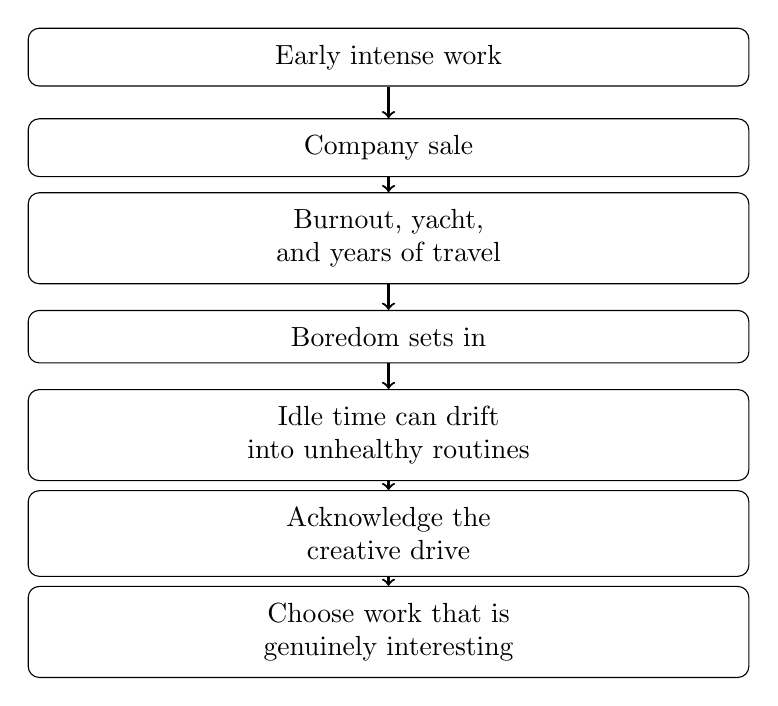
\begin{tikzpicture}[
  box/.style={
    draw,
    rounded corners,
    align=center,
    text width=0.72\linewidth,
    inner sep=6pt
  },
  arrow/.style={->, thick}
]
\node[box] (work) at (0,0) {Early intense work};
\node[box] (sale) at (0,-1.15) {Company sale};
\node[box] (travel) at (0,-2.30) {Burnout, yacht,\\and years of travel};
\node[box] (boredom) at (0,-3.55) {Boredom sets in};
\node[box] (risk) at (0,-4.80) {Idle time can drift\\into unhealthy routines};
\node[box] (creative) at (0,-6.05) {Acknowledge the\\creative drive};
\node[box] (interest) at (0,-7.30) {Choose work that is\\genuinely interesting};

\draw[arrow] (work) -- (sale);
\draw[arrow] (sale) -- (travel);
\draw[arrow] (travel) -- (boredom);
\draw[arrow] (boredom) -- (risk);
\draw[arrow] (risk) -- (creative);
\draw[arrow] (creative) -- (interest);
\end{tikzpicture}
\caption{Editorial reconstruction of the interview's causal sequence. The exit does not end the creative problem; it changes the form of the problem.}
\end{figure}

The whole passage can now be read as one movement:

\begin{align}
\text{work} &\longrightarrow \text{exit},\\
\text{exit} &\longrightarrow \text{freedom},\\
\text{freedom without structure} &\longrightarrow \text{boredom},\\
\text{boredom, handled well} &\longrightarrow \text{interesting creative work}.
\end{align}

This is the useful reconstruction. The speaker is not recommending endless company formation for its own sake. He is describing how, for him, motivation returned when creation was attached to interest rather than to raw grind.

\section{Summary}

The interview begins with motivation and ends with fit. The speaker first rejects the idea that relentless work simply continues forever: he worked hard young, sold the company, and burned out. He then tried the post-exit dream seriously, buying a large yacht and traveling for years. The pivot came when leisure became boredom, and boredom became a risk state.

The practical answer is to acknowledge the creative drive and choose work that is genuinely interesting. For the larger entrepreneurship book, this belongs with resilience and judgment. Motivation after success is not just a matter of forcing effort; it is the discipline of distinguishing exhaustion from freedom, freedom from direction, and direction from mere busyness.